\chapter{Note Set Data Container Specification}
\label{chap:technicaldocu}

\section{Note Set Annotation Specification}

\subsection{Motivation}
As already mentioned, we introduce Note Sets as a container for notes which are equivalent with respect to a yet to be defined annotation, the labeling of the set. Since the Note Set itself is basically just a set of IDs or keys, all substantial information will be in the annotation. The first challenge is to select the properties which should be part of the annotation. The second is the question of how to persist the annotation within the Note Set. Since we do not want to introduce a new Note container format, it's not possible to add the annotation as a sort of header in an XML or JSON format. This would mean that a new format has been introduced and some kind of schema defined for it. \par
The only option that remains is thus to store the set's annotation within the filename itself when exporting a Note Set to disk. For this a special file format string has to be introduced (see below).
\subsection{Criteria for selecting annotational elements}
The selection of the elements which should be part of the annotation was overall not that easy, on the one hand because there are hundreds of properties in a NIF file and we want to be as specific as possible, on the other hand, a Note Set's annotation should be as simple as possible, namely because we want to persist the annotation in a Note Set's filename, which ideally should be a readable and not too long string.
Finally after having consulted with the adaptation specialist team, the selection was done by the following criteria: The mandatory properties are properties which are needed to identify notes in MCM, the same criteria needed when mapping a loaded note to a reference note in a CDF. The optional properties (with the exception of comment) are criteria for which it is very likely that a user wants to split or filter a set of notes by when analyzing or training algorithms.
\subsection{Mandatory Elements of the Note Set Annotation}
The following attributes form the mandatory part of the Note Set's annotation. These are all derived from properties set in the NOTEMSG2 chunk of the NIF file. 
\begin{description}
  \item[Currency] Corresponds to the ISO string matching the the numeric ISOCODE value in the NOTEMSG2 Chunk.
  \item[IsoGroup] 
  \item[Emission] Emission of the notes in the Note Set, corresponds to the value of the Chunk EMISSION in NOTEMSG2
  \item[Orientation] Orientation of the notes in the Note Set, corresponds to to ORIENTATION in NOTEMSG2
\item[Type] NoteType (indicating the reference note this note is matched to by the CDF which was used in recording). For currencies like, GBP with different printers (for example HKD\footnote{Hong Kong Dollar} or GBP\footnote{Great Britain Pound}), this type is necessary to identify a note. For other currencies with only one printer, like CHF, denomination and emission is usually enough to identify a note.
\end{description}

\subsection{Optional Elements of the Note Set Annotation}
The following attributes are optional elements of a Note Set Annotation. They are not identifying properties but qualify a note (set).

\begin{description}
\item[Class] Corresponds to the value CATEGORY in NOTEMSG2 Chunk and is an attribute for authenticity and fitness of a banknote, for example, Category 4a notes are authentic and fit notes, Category 2 are counterfeits. It's a likely use case that a user would want to split notes across a currency by category to train and analyze fitness and security algorithms. 
\item[Security and Fitness flags Flags] Security and Fitness Flags are set by certain algorithms and indicate that a note might be classified as unfit or counterfeit. For example, the fitness flag STAIN indicates that the note has some kind of smudging, the security flag ROBBERY\_INK indicates that the presence of robbery ink was detected. 
\item[Reject Reason] This is an enum value found corresponding to the value REJECT\_REASON in NOTEMSG2 chunk. It indicates the reason why a note was rejected or that it was not rejected.
\item [Comment] This is an optional comment added by the user and the only value which does not come from the NIF file
\end{description}

\subsection{Specifying the file format string}
As already stated, the Note set's annotation is to be converted into a filename when exporting a Note Set to ASCII. The file format string to be constructed has to be readable, complete and indicate the optionality of properties, i.e. distinguish the optional properties from the mandatory ones. Finally, the goal is to codify the format into a regular expression and implement an annotation parser in the python noteset library \emph{pynoteset}.
\subsubsection{Preliminary Decisions}
\begin{itemize}
\item Generic placeholder for non-specified mandatory properties: Since we allow Note Sets to be merged, we have to anticipate the scenario where e.g. a Note Set contains notes of various denominations. Therefore we need a placeholder for all mandatory properties indicating the state of 'Undefined' or mixed. This placeholder is 'XXX' for currencies and isogroups and 'X' otherwise, a practice which is already in use in the recording of note data and thus one that users are already familiar with. 
\item Allowing of both upper- and lowercase spelling: While it is common to use uppercase notation for currency ISO codes, we will allow both upper- and lowercase notation to make the already fairly complicated string format less restrictive.
\end{itemize}



\subsection{Security and Fitness Flags}

Security and Fitness Flags are set by certain algorithms and indicate that a note might be classified as unfit or counterfeit. For example, the fitness flag STAIN indicates that the note has some kind of smudging, the security flag ROBBERY\_INK indicates that the presence of robbery ink was detected. \par
Since it is a probable use case that one might want to generate set of notes where a specific flag is set (to train the algorithm which sets said flag), it's important that flags be persisted in a note set's annotation as well. \par
The problem is that there could be multiple flags set for the notes in one set, say all notes with flags STAIN and INK. In practice, this use case is not too likely, but we want to allow this scenario to remain as generic as possible. We don't, however, want the annotation string to become too long and hard to read. 
Apart from impeded readability, another problem is that we now have in addition to the comment property a second optional property which has a multplicity of 1...n. This makes correct parsing of an annotation string a bit more difficult. 
\begin{figure}[hbt!]
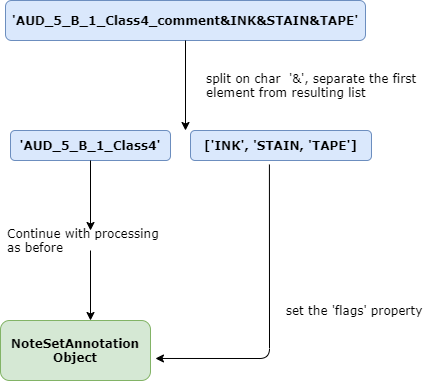
\includegraphics[width=0.5\columnwidth]{images/notesetannotation_flags.png}
\caption{Persisting flags in Note Set filename}\label{fig:awesome_image1}
\end{figure}